

\begin{center}
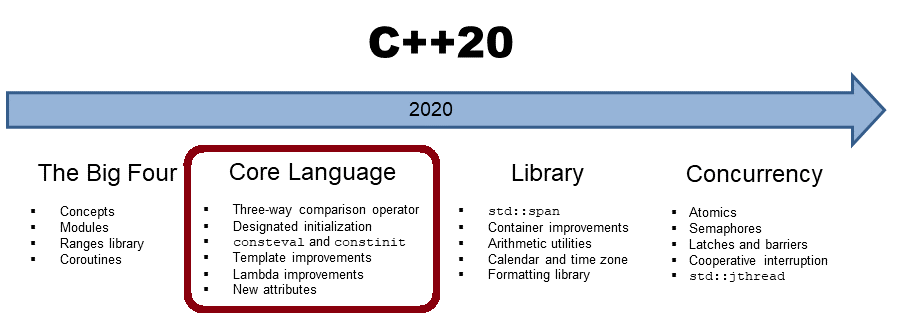
\includegraphics[width=1.0\textwidth]{content/2/chapter3/images/4.png}\\
\end{center}

\subsubsubsection{3.2.1\hspace{0.2cm}三向比较操作符}

三向比较操作符<=>,或宇宙飞船操作符,确定对于两个值A和B的大小关系, A < B,A == B,或A > B。

通过将三向比较操作符声明为default,编译器将尝试为该类自动生成关系操作符。在本例中,将得到所有六个比较运算符:==、!=、<、<=、>和>=。

\begin{lstlisting}[style=styleCXX]
struct MyInt {
	int value;
	MyInt(int value): value{value} { }
	auto operator<=>(const MyInt&) const = default;
};
\end{lstlisting}

编译器生成的操作符<=>执行字典比较,从基类开始,按照声明顺序考虑所有非静态数据成员。下面的复杂例子,来自于Microsoft的博客:\href{https://devblogs.microsoft.com/cppblog/simplify-your-code-with-rocket-science-c20s-spaceship-operator/}{使用“航天学”简化代码:C++20的宇宙飞船操作符}。

\subsubsubsection{3.2.2\hspace{0.2cm}指定初始化}

\begin{lstlisting}[style=styleCXX]
struct Basics {
	int i;
	char c;
	float f;
	double d;
	auto operator<=>(const Basics&) const = default;
};

struct Arrays {
	int ai[1];
	char ac[2];
	float af[3];
	double ad[2][2];
	auto operator<=>(const Arrays&) const = default;
};

struct Bases : Basics, Arrays {
	auto operator<=>(const Bases&) const = default;
};

int main() {
	constexpr Bases a = { { 0, 'c', 1.f, 1. },
		{ { 1 }, { 'a', 'b' }, { 1.f, 2.f, 3.f }, { { 1., 2. }, { 3., 4. } } } };
	constexpr Bases b = { { 0, 'c', 1.f, 1. },
		{ { 1 }, { 'a', 'b' }, { 1.f, 2.f, 3.f }, { { 1., 2. }, { 3., 4. } } } };
	static_assert(a == b);
	static_assert(!(a != b));
	static_assert(!(a < b));
	static_assert(a <= b);
	static_assert(!(a > b));
	static_assert(a >= b);
}
\end{lstlisting}

假设这段代码中最复杂的不是太空船操作符,而是使用聚合初始化初始化Base。聚合初始化意味着若所有成员都是public,则可以直接初始化类类型(class、struct或union)的成员。所以,可以使用带括号的初始化列表,如示例所示。

讨论指定初始化之前,先来详细介绍一下聚合初始化。先来看一个简单的例子。

\begin{lstlisting}[style=styleCXX]
struct Point2D{
	int x;
	int y;
};

class Point3D{
	public:
	int x;
	int y;
	int z;
};

int main(){
	std::cout << "\n";
	Point2D point2D {1, 2};
	Point3D point3D {1, 2, 3};
	std::cout << "point2D: " << point2D.x << " " << point2D.y << "\n";
	std::cout << "point3D: " << point3D.x << " "
	<< point3D.y << " " << point3D.z << "\n";
	std::cout << '\n';
}
\end{lstlisting}

输出为:

\begin{center}
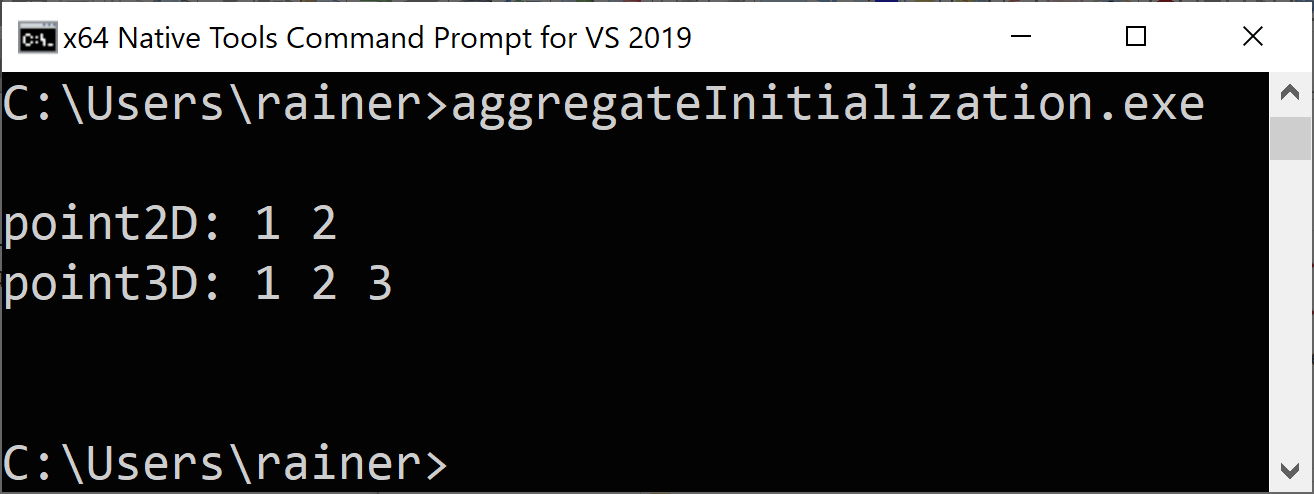
\includegraphics[width=0.6\textwidth]{content/2/chapter3/images/5.png}
\end{center}

因为可以交换构造函数参数,所以聚合初始化非常容易出错,而且不太会注意到,所以显式方式要好于隐式方式。再来看下\href{https://en.wikipedia.org/wiki/C99}{C99}(现在是C++标准的一部分)中的指定初始化:

\begin{lstlisting}[style=styleCXX]
struct Point2D{
	int x;
	int y;
};

class Point3D{
public:
	int x;
	int y;
	int z;
};

int main(){

	Point2D point2D {.x = 1, .y = 2};
	// Point2D point2d {.y = 2, .x = 1}; // error
	Point3D point3D {.x = 1, .y = 2, .z = 2};
	// Point3D point3D {.x = 1, .z = 2} // {1, 0, 2}


	std::cout << "point2D: " << point2D.x << " " << point2D.y << "\n";
	std::cout << "point3D: " << point3D.x << " " << point3D.y << " " << point3D.z
		      << "\n";

}
\end{lstlisting}

Point2和Point3D实例的参数显式命名,该程序的输出与前一个程序的输出完全相同。注释掉的第16行和第18行非常有趣。第16行会报错,因为指示符的顺序与数据成员的声明顺序不匹配。至于第18行,y的指示符不见了,所以y会初始化为0,等效于使用带括号的初始化列表\{1,0,2\}。

\subsubsubsection{3.2.3\hspace{0.2cm}consteval和constinit}

C++20中新增的consteval说明符创建了一个即时函数。所谓即时函数,每次调用该函数都会生成一个编译时常量表达式。即时函数是隐式constexpr函数,但不一定是constexpr函数。

\begin{lstlisting}[style=styleCXX]
consteval int sqr(int n) {
	return n*n;
}
constexpr int r = sqr(100); // OK

int x = 100;
int r2 = sqr(x); // Error
\end{lstlisting}

因为x不是一个常量表达式,最后的赋值会出错,因此不能在编译时执行sqr(x)。

constinit(详见4.5.2节)确保静态存储时间段或线程存储时间段的变量,在编译时初始化。静态存储时间段意味着对象在程序开始时分配,在程序结束时释放。线程存储时间段,意味着对象的生存期与线程的生存期绑定。

constinit确保在编译时对这类变量(静态存储时间段或线程存储时间段)进行初始化。不过,constinit并不意味着常量。

\subsubsubsection{3.2.4\hspace{0.2cm}模板的改进}

C++20对模板编程提供了各种改进。泛型构造函数是一种万能构造函数,可以用任何类型使用。

\hspace*{\fill} \\ %插入空行
\noindent
\textbf{隐式和显式泛型构造函数}
\begin{lstlisting}[style=styleCXX]
struct Implicit {
	template <typename T>
	Implicit(T t) {
		std::cout << t << '\n';
	}
};

struct Explicit {
	template <typename T>
	explicit Explicit(T t) {
		std::cout << t << '\n';
	}
};

Explicit exp1 = "implicit"; // Error
Explicit exp2{"explicit"};
\end{lstlisting}

隐式类的构造函数很泛型,通过将关键字explicit放在构造函数前面,就像显式构造函数一样,从而隐式转换不再有效。

\subsubsubsection{3.2.5\hspace{0.2cm}Lambda表达式的改进}

Lambda在C++20中进行了许多改进,可以有模板参数,可以在未求值的上下文中使用,无状态的Lambda也可以默认构造和复制赋值。此外,编译器现在可以检测何时隐式复制this指针。

若想定义一个只接受std::vector的Lambda表达式,模板参数可以这样写:

\begin{lstlisting}[style=styleCXX]
auto foo = []<typename T>(std::vector<T> const& vec) {
		// do vector-specific stuff
	};
\end{lstlisting}

\subsubsubsection{3.2.6\hspace{0.2cm}新属性}

C++20有了新的属性,包括[[likely]]和[[unlikely]]。这两个属性都可以给优化器一些提示,指定哪个执行路径更可能或更不可能(可以更好的进行分支预测)。

\hspace*{\fill} \\ %插入空行
\noindent
\textbf{属性[[likely]]}
\begin{lstlisting}[style=styleCXX]
for(size_t i=0; i < v.size(); ++i){
	if (v[i] < 0) [[likely]] sum -= sqrt(-v[i]);
	else sum += sqrt(v[i]);
}
\end{lstlisting}